\documentclass[12pt]{extarticle} 
\usepackage{unicode-math}
\usepackage{amsthm,graphicx,xcolor,natbib,enumitem,booktabs,tabularx}
%\usepackage[paperwidth=126mm, paperheight=96mm, top=5mm, bottom=5mm, right=5mm, left=5mm]{geometry}
\usepackage[margin=1cm]{geometry}
\pagenumbering{gobble}

\usepackage[BoldFont,SlantFont]{xeCJK}  
\xeCJKsetemboldenfactor{2}
\setCJKmainfont{cwTeX Q Yuan Medium}
\newcommand{\ds}{\displaystyle}
\newcommand{\ie}{\,\Longrightarrow\,}
\newcommand{\ifff}{\,\Longleftrightarrow\,}
\newcommand{\mi}{\mathrm{i}}
\DeclareMathOperator*{\dom}{dom}
\DeclareMathOperator*{\codom}{codom}
\DeclareMathOperator*{\ran}{ran}
\newcommand{\floor}[1]{\lfloor #1 \rfloor}
\newcommand{\ceil}[1]{\lceil #1 \rceil}

% figure --> 圖
\renewcommand{\appendixname}{附錄}
\renewcommand{\figurename}{圖}
\renewcommand{\tablename}{表}
\renewcommand{\refname}{參考文獻}

\usepackage{hyperref}
\hypersetup{
    colorlinks,
    linkcolor={red!50!black},
    citecolor={blue!60!black},
    urlcolor={blue!60!black}
    %urlcolor={blue!80!black}
}

\theoremstyle{definition}
\newtheorem*{dfn}{定義}
\newtheorem*{prp}{性質}
\newtheorem*{thm}{定理}
\newtheorem*{ex}{例}
\newtheorem*{sol}{解}
\newtheorem*{prf}{證}

%\setenumerate{label=(\roman*),itemsep=1pt,topsep=3pt}
\newcommand{\myline}{\noindent\makebox[\linewidth]{\rule{\paperwidth}{0.4pt}}}
%\newcommand{\myline}{\textcolor[RGB]{220,220,220}{\rule{\linewidth}{1pt}}}

\usepackage{tikz}
\usetikzlibrary{arrows.meta,angles,quotes}
\usepackage{pgfplots}
% axis style, ticks, etc
\pgfplotsset{every axis/.append style={
                   label style={font=\fontsize{4}{4}\selectfont},
                   tick label style={font=\fontsize{4}{4}\selectfont}  
               },
            }
\renewcommand\tabularxcolumn[1]{m{#1}}

\begin{document}
\title{\texorpdfstring{\vspace{-16mm} 反三角函數}{反三角函數}} 
\author{\vspace{-5em}}
\date{\vspace{-5em}}
\maketitle

\vspace{1em}
\begin{dfn}
  在以下定義域上之三角函數為嵌射:
  \begin{align*}
    &\sin x: \big[-\frac{\pi}{2}, \frac{\pi}{2}\big]\to[-1, 1] &\csc x: \big(0, \frac{\pi}{2}\big]\cup\big(\pi, \frac{3\pi}{2}\big]\to(-\infty, -1]\cup[1,\infty) \\
    &\cos x: \big[0, \pi\big]\to[-1, 1] &\sec x: \big[0, \frac{\pi}{2}\big)\cup\big[\pi, \frac{3\pi}{2}\big)\to(-\infty, -1]\cup[1,\infty) \\
    &\tan x: \big(-\frac{\pi}{2}, \frac{\pi}{2}\big)\to(-\infty, \infty) &\cot x: \big(0, \pi\big)\to(-\infty, \infty)\qquad\qquad
  \end{align*}
  故存在反三角函數:
  \begin{align*}
   &\sin^{-1} x: [-1, 1]\to\big[-\frac{\pi}{2}, \frac{\pi}{2}\big] &\csc^{-1} x: (-\infty, -1]\cup[1,\infty)\to\big(0, \frac{\pi}{2}\big]\cup\big(\pi, \frac{3\pi}{2}\big] \\
   &\cos^{-1} x: [-1, 1]\to\big[0, \pi\big] &\sec^{-1} x: (-\infty, -1]\cup[1,\infty)\to\big[0, \frac{\pi}{2}\big)\cup\big[\pi, \frac{3\pi}{2}\big) \\
   &\tan^{-1} x: (-\infty, \infty)\to\big(-\frac{\pi}{2}, \frac{\pi}{2}\big) &\cot x: (-\infty, \infty)\to\big(0, \pi\big)\qquad\qquad
 \end{align*}
\end{dfn}

\begin{prp}
  \begin{itemize}
    \item[]
    \item 當 $\ds-\frac{\pi}{2}\leqslant x\leqslant\frac{\pi}{2}$,$\sin^{-1}(\sin x) = x$;當 $\ds 0\leqslant x\leqslant\pi$,$\cos^{-1}(\cos x) = x$。
    \item 當 $\ds-1\leqslant x\leqslant1$,$\sin(\sin^{-1} x) = x$,$\cos(\cos^{-1} x) = x$。
    \item $\sin^{-1}(-x) = -\sin^{-1}x$;$\cos^{-1}(-x) = \pi - \cos^{-1}x$。
  \end{itemize}
\end{prp}

\vspace{-1cm}
\begin{figure}[!htbp]
  \centering
  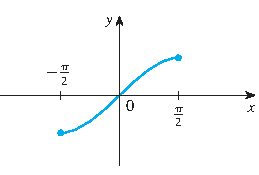
\includegraphics[scale=1.44,page=1]{fig/trig.pdf}
  \includegraphics[scale=1.2,page=2]{fig/trig.pdf}
  \caption{$y = \sin x$,$y = \sin^{-1} x$}
\end{figure}

\vspace{-1cm}
\begin{figure}[!htbp]
  \centering
  \includegraphics[scale=1.44,page=3]{fig/trig.pdf}
  \includegraphics[scale=1.2,page=4]{fig/trig.pdf}
  \caption{$y = \cos x$,$y = \cos^{-1} x$}
\end{figure}

\vspace{-1cm}
\begin{figure}[!htbp]
  \centering
  \includegraphics[scale=1.2,page=5]{fig/trig.pdf}
  \includegraphics[scale=1.2,page=6]{fig/trig.pdf}
  \caption{$y = \tan x$,$y = \tan^{-1} x$}
\end{figure}

\newpage

\begin{ex} 
  \begin{align*}
    &\sin^{-1}\frac{\sqrt{3}}{2} = \frac{\pi}{3}\qquad &\cos^{-1}\frac{-1}{2} = \frac{2\pi}{3}\quad\text{($[0,\,\pi]$ 對稱)}\\
    &\tan^{-1}1 = \frac{\pi}{4}\qquad&\cos\big(\sin^{-1}\frac{3}{5}\big) = \frac{4}{5}\qquad\qquad
  \end{align*}
\end{ex}

\begin{ex}
  若 $\ds\alpha = \sin^{-1}\frac{2}{3}$,求 $\cos\alpha$,$\tan\alpha$,$\cot\alpha$,$\sec\alpha$,$\csc\alpha$。
\end{ex}

\begin{sol}
  $\ds\cos\alpha = \frac{\sqrt{5}}{3}$,$\ds\tan\alpha = \frac{2}{\sqrt{5}}$,$\ds\cot\alpha = \frac{\sqrt{5}}{2}$,$\ds\sec\alpha = \frac{3}{\sqrt{5}}$,$\ds\csc\alpha = \frac{3}{2}$。
\end{sol}

%\begin{ex}
%  若 $\ds f(x) = \frac{1}{\sin^{-1}\big(\frac{1}{x}\big)}$,求 $\dom{f}$。
%\end{ex}
%
%\begin{sol}
%  $\dom f = \big\{x\,|\, -1\leqslant\frac{1}{x}\leqslant 1\big\} = (-\infty,-1]\,\cup\,[1,\infty)$。
%\end{sol}
%
%\begin{ex}
%  令 $\ds f(x) = \sin(\sin^{-1} x)$,$\ds g(x) = \sin^{-1}(\sin x)$,求 $\dom{f}$,$\dom{g}$ 與其圖形。
%\end{ex}
%
%\begin{sol}
%  \begin{itemize}
%    \item[]
%    \item $\dom f = \dom{\sin^{-1}} = [-1, 1]$;$f(x) = x$,$\forall\,x\in[-1, 1]$。
%    \item $\ds\dom g = \mathbb{R}$;$\ds g(x) = \begin{cases} -x + (2n + 1)\,\pi & x\in[(2n + \frac{1}{2})\,\pi,\, (2n + \frac{3}{2})\,\pi) \\ x - (2n + 2)\,\pi & x\in[(2n + \frac{3}{2})\,\pi,\, (2n + \frac{5}{2})\,\pi)\end{cases}\quad n\in\mathbb{Z}$。
%    %\vspace{-1cm}
%    \begin{figure}[!htbp]
%      \centering
%      \begin{tikzpicture}[scale=2.6]
%        \begin{axis}%
%          [grid=both,
%           unit vector ratio*=1 1 1,
%           minor tick num=1,
%           grid style={line width=.1pt, draw=gray!10},
%           major grid style={line width=.2pt,draw=gray!50},
%           axis lines=middle,
%           xtick={-6.28318, -4.7123889, -3.14159, -1.5708, 1.5708, 3.14159, 4.7123889, 6.28318},
%           xticklabels={$-2\pi$, $-\frac{3\pi}{2}$, $-\pi$, $-\frac{\pi}{2}$, $\frac{\pi}{2}$, $\pi$, $\frac{3\pi}{2}$, $2\pi$},
%           ytick={-1.5708, 1.5708},
%           yticklabels={$-\frac{\pi}{2}$, $\frac{\pi}{2}$},
%           x tick label style={yshift=0.3em},
%           y tick label style={xshift=0.3em},
%           enlargelimits={abs=0.5}
%          ]
%          \addplot[domain=-2*pi:2*pi,samples=3000,smooth,cyan] {rad(asin(sin(deg(x))))};
%        \end{axis}
%      \end{tikzpicture}
%      \caption{$g(x) = \sin^{-1}(\sin x)$}
%    \end{figure}
%  \end{itemize}
%\end{sol}

\begin{ex}
  將 $\ds\sin(\cos^{-1} x)$ 與 $\tan(\cos^{-1} x)$ 化簡為 $x$ 的(不含三角函數之)表示式,其中 $-1\leqslant x\leqslant 1$。
\end{ex}

\begin{sol}
  令 $\ds u =\cos^{-1}x$,則 $\ds0\leqslant u\leqslant\pi$,$\cos u = x$,$\ds\sin u = +\sqrt{1 - x^2}$,$\ds\tan u = \frac{\sqrt{1 - x^2}}{x}$。
\end{sol}

\begin{ex} 
  $\ds\cos(\sin^{-1} x) = \sqrt{1 - x^2}$,$\ds\quad\sin(\tan^{-1} x) = \frac{x}{\sqrt{1 + x^2}}$,$\ds\quad\sin(2\tan^{-1} x) = \frac{2x}{1 + x^2}$。
\end{ex}

\begin{ex}
  將 $\ds \sin(\cos^{-1} x + \tan^{-1}y)$ 化簡為 $x$,$y$ 的(不含三角函數之)表示式,其中 $-1\leqslant x\leqslant 1$,$y\in\mathbb{R}$。
\end{ex}

\begin{sol}
  令 $\ds u =\cos^{-1}x$,$\ds v=\tan^{-1} y$,則 $\cos u = x$,$\tan v = y$,由此 $\ds\sin u = \sqrt{1 - x^2}$,$\ds\cos v = \frac{1}{\sqrt{1 + y^2}}$,$\ds\sin v = \frac{y}{\sqrt{1 + y^2}}$;原式為 $\ds\sin(\cos^{-1} x + \tan^{-1}y) = \sin(u + v) = \sin u\cos v + \cos u\sin v = \sqrt{1 - x^2}\cdot\frac{1}{\sqrt{1 + y^2}} + x\cdot\frac{y}{\sqrt{1 + y^2}}$。
\end{sol}

\begin{ex}
  證明 $\ds\cos^{-1}(1 - 2x^2) = 2\sin^{-1}x$,$0\leqslant x\leqslant 1$。
\end{ex}

\begin{sol}
  令 $\ds u = \sin^{-1}x$,則 $\ds\cos^{-1}(1 - 2x^2) = \cos^{-1}(1 - 2\sin^2u) = \cos^{-1}(\cos 2u) = 2u = 2\sin^{-1}x$。
\end{sol}

\begin{ex}
  解 $\ds2\sin^{-1} x + \cos^{-1}x = \pi$。
\end{ex}

\begin{sol}
  令 $\ds\sin^{-1}x = u$,$\ds\cos^{-1}x = v$,則 $\ds\sin u = \cos v = x$,$\ds\cos u = \sin v = \sqrt{1 - x^2}$。方程式兩邊取 $\cos$ $\ds\ie\cos(2u + v) = -1 \ie \cos2u\cos v - \sin2u\sin v = (1 - 2\sin^2u)\cos v - 2\sin u\cos u\sin v = -1 \ie (1 - 2x^2)x - 2 x(1 - x^2) = -1 \ie x = 1$。
\end{sol}

\end{document}
